%% This is an example first chapter.  You should put chapter/appendix that you
%% write into a separate file, and add a line \include{yourfilename} to
%% main.tex, where `yourfilename.tex' is the name of the chapter/appendix file.
%% You can process specific files by typing their names in at the 
%% \files=
%% prompt when you run the file main.tex through LaTeX.
\chapter{Stochastic Traceback Algorithm and Improvements}

\section{Introduction}

The stochastic traceback algorithm was introduced by Ye Ding and
Charles Lawrence \cite{ding2003statistical} as a means to explore the
energy landscape of RNA by sampling structures according to their
Boltzmann probabilities. This was important because the minimum free
energy structure was very sensitive to errors in the parameters of the
free energy model, and although algorithms existed for generating
suboptimal structures, they either sampled a very limited set of
states \cite{zuker1989finding}, or had exponential runtime and the
output did not have the same distribution as the physical ensemble of
states \cite{wuchty199complete}. Structures sampled according to this
algorithm can be clustered into macrostates, whos properties can be
examined.

The method first computes the partition function, then it ``traces
back'' over the contents of the tables calculated during that
algorithm. Specifically, the tables $Q(i,j)$, $Q^b(i,j)$, etc. now
contain information about the conditional probabilities of bases
pairing. Starting from a bare, undetermined strand at the top of the
recurrence relations, the stochastic traceback samples pairs between
bases until a structure is formed such that its probability of it
being created by the algorithm is equal to its boltzmann weight
$e^{-E(s)/RT}/Z$.

The general principle of the backwards trace is that,
presented with several possibilities for the structure along a
sequence from $i$ to $j$, the sampling probability for a case is the
contribution to the partition function by that case's partition
function. For example, since the partition function $Q(i, j)$ is defined:
\begin{equation}
Q(i,j) = \overbrace{e^{-b(j-i+1)/RT}}^{\text{empty}} + \overbrace{\sum_{\substack{ d,e \\ i \leq d < e \leq j}}Q(i, d - 1) Q^b(d, e) e^{-b(j-e)/RT}}^{\text{rightmost pair}},
\end{equation}
during a stochastic traceback the probability of sampling a pairless
strand, and the probability of drawing a rightmost pair $(d,e)$ and
recursing from there are:
\begin{align}
P(\text{empty} | i, j) &= \frac{e^{-b(j-i+1)/RT} }{Q(i,j)} \\ 
P(\text{pair } (d,e) | i, j ) &= \frac{ Q(i, d-1) Q^b(d,e) e^{-b(j-e)/RT}}{Q(i,j)}. 
\end{align}
Notice that when summed together for every possible case of $(d,e)$,
the numerator becomes the definition of $Q(i,j)$, so these
probabilities are naturally normalized. Likewise, since $Q^b(i,j)$ is
defined as 
\begin{equation}
\begin{split}
 Q^b(i, j) =& \overbrace{e^{-E_h(i,j)/RT}}^{\text{hairpin}} +
 \overbrace{e^{-E_s(i, j)/RT} Q^b(i+1, j-1)}^{\text{stack}} \\ 
& + \overbrace{\sum_{\substack{d,e \\ i < d< e< j}} e^{-E_i(i, d, e, j)/RT}Q^b(d,e)}^{\text{internal}} \\ 
& + \overbrace{e^{-a/RT} \sum_{\substack{d,e \\ i < d< e< j}} Q(i+1, d-1) Q^b(d,e) e^{-b(j-e-1)/RT}}^{\text{multiloop}}.
\end{split}
\end{equation}
The probability of sampling a hairpin, stack loop, internal loop, and multiloop are:
\begin{align}
P(\text{hairpin} | i, j) &= \frac{ e^{-E_h(i,j)/RT} } { Q^b(i,j) } \\
P(\text{stack} | i, j ) &= \frac{ e^{-E_s(i,j)/RT} Q^b(i+1, j-1) } {Q^b(i,j)}  \\
P(\text{internal } (d, e) | i, j) &= \frac{e^{-E_i(i, d, e, j)/RT} Q^b(d,e)}{Q^b(i,j) }\\
P(\text{multi }(d,e) |i, j ) &= \frac{ e^{-a/RT} Q(i + 1, d-1) Q^b(d,e) e^{-b(j-e-1)/RT} } { Q^b(i,j)} 
\end{align}
Notice for the same reason as before, all the probabilities for the
$Q^b$ recursion sum to one. In general, the stochastic traceback can
be readily understood by examining the recurrence relation figures
from chapter 2: Figure \ref{fig:recurrenceRelationsQij} and Figure
\ref{fig:recurrenceRelationsQbij}. We start at the $Q$ recursion for
the strand, we may pick a pair and add it to the structure, but in
general, for every pair added we recurse down to $Q^b$ on that region
to determine the structure below that pair. For every structure left
undetermined, we use the probabilities from $Q$ to determine that
structure and so on. 

\begin{figure}
\centering
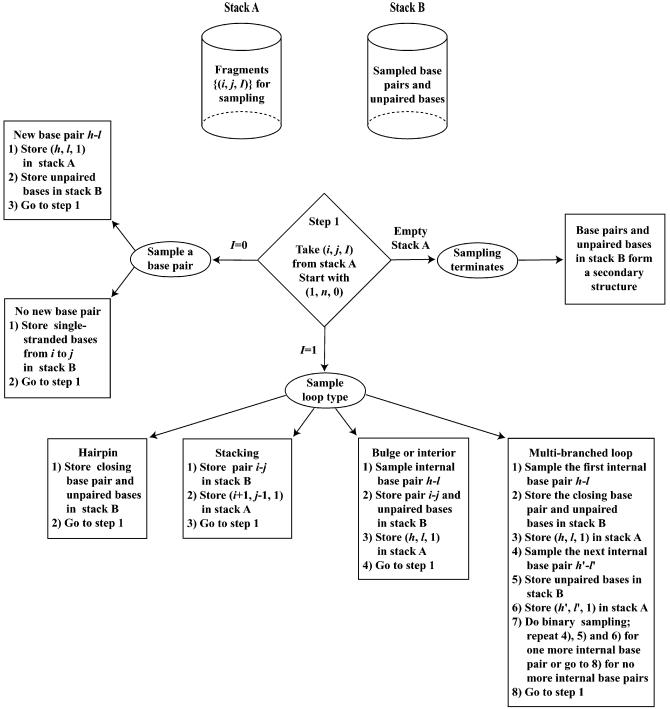
\includegraphics[width=\textwidth]{stochastic-alg-diagram.jpg}
\caption{Flowchart of the algorithm from Ding and Lawrence's paper
  \cite{ding2003statistical}. Basically: if we are on a $Q(i,j)$
  recursion, sample either an empty section or a rightmost pair. For
  $Q^b$ choose a loop type and corresponding pairs if
  applicable. After both cases recurse down appropriately so that
  $Q^b$ is drawn for any pair created and $Q$ for any open region.}
\label{fig:stoch-flowchart}
\end{figure}

The algorithm's implementation uses two stack data structures. A stack
can be thought of as a literal "stack", like papers stacked on a desk,
except instead of paper their are items of data. There are two basic
operations, one to put an item on the top of the stack, and another to
retrieve an item off the top. These are called "push" and "pop"
operations, respectively, in Computer Science. The data items we will
be pushing on to the first stack, A, are of the form $\{(i,j), b\}$
where $i$ and $j$ are indexes along the strand and $b$ is either
$true$ if we have determined that $i$ and $j$ are paired, or $false$
otherwise. The second stack, B, is where we'll collect pairs and
unpaired bases for one sample.

\begin{figure}[h]
\bfseries\small
The initialization of the algorithm is to push $\{(1, n), false\}$
onto the stack. From there the algorithm repeats the following steps:
\begin{enumerate}
\item Pop an element, $\{i, j, b\}$ off stack A.
\item Case b is $false$:
\begin{enumerate}
\item ($Q(i,j)$ recursion) Pick empty or pair $(k,l)$ with
  probabilities listed above. If empty, push all pairs on $[i, j]$
  inclusive onto B as unpaired bases, if not push $\{(d, e), true\}$
  and $\{(i, d-1), false\}$ onto A.
\end{enumerate}
\item Case b is $true$:
\begin{enumerate}
\item ($Q^b(i,j)$ recursion) Choose what type of loop $(i,j)$ is from
  the probabilities listed above.
\item Push the appropriate elements onto the stack for that loop type,
  see Figure \ref{fig:stoch-flowchart}.
\end{enumerate}
\item If stack A is empty, the pairs and unpaired bases in stack B
  become a sampled structure. Reinitialize for additional samples.
\end{enumerate}

\caption{The stochastic traceback algorithm is implemented by pushing
  the recursive elements back onto the stack to sample a full structure. }
\label{fig:stochastic-pseudocode}
\end{figure}

The algorithm displayed in Figure \ref{fig:stochastic-pseudocode} is
what gets the job done. The probability of the structure is equal to
the product of the probabilities that determined its pairs and empty
regions, but if you follow the recursion all the way down you see that
this results in just the boltzmann factor for the structure:
\begin{equation}
P(s) = \prod_{\text{cases}} \frac{P(\text{case})}{Q(\text{case})} =
\frac{1}{Z} e^{-E(s)/RT}.
\end{equation}

\section{Motivation}

In the past 10 years, the stochastic traceback algorithm has become an
increasingly central part of RNA secondary structure prediction
algorithms \cite{mathews2006revolutions}. This is because they present
many advantages over the minimum free energy prediction. It can be
shown that the minimum free energy state, even though it is the most
probable state, can still have astronomically unlikely probabilities
on average for typical strands of reasonable length (Figure
\ref{fig:probMFE}). The more important concept in understanding the
physical behavior of an RNA strand is therefore the overall shape of
the energy landscape. Althogh the probability of any individual
structure might be infinitesimally small, there can be shown to be
relatively few large basins containing clusters of similar foldings.
The consensus structures and the difference between the consensus
structures of these basins define the function of the RNA molecule.

The way the stochastic algorithms probe that is by providing
structures to group into these basins, and since the stochastic
traceback algorithm samples states with the exact probability defined
by the partition function, we know that the macrobehavior of these
samples match what we would probably see in reality. There is one
catch and that is statistical error. However, the error can be reduced
and the landscape can be further explored the more stochastic samples
we make.

The need to sample large numbers of secondary structures makes a
speedup very convenient, and that is what motivates our current
expedition.

\section{Adding Efficiency}

Taking advantage of the empirical fact that the number of probable
base pairs for an RNA strand tend to grow very slowly, we can restrict
our traceback to only explore bases that we know can pair with one
another. This is as simple as replacing the old recurrence relations
with the new ones. For example during a $Q(i,j)$ state of the
recursion there would be probabilities of:
\begin{align}
P(\text{empty} | i, j) &= \frac{e^{-b(j-i+1)/RT}}{Q(i,j)}\\
P(\text{goto } Q^m | i, j) &= \frac{Q^m(i, j) }{Q(i, j) }.
\end{align}
For a $Q^m$ state:
\begin{align}
P(\text{continue} | i, j) = \frac{Q^m(i, j -1) e^{-b/RT}} {Q^m(i, j) }\\
P(\text{pair } (k, j) | i, j) = \frac{Q(i, k - 1) Q^b(k, j) } {Q^m(i,j) }.
\end{align}
And finally for $Q^b(i, j)$:
\begin{align}
P(\text{hairpin} | i, j) &= \frac{ e^{-E_h(i,j)/RT} } { Q^b(i,j) } \\
P(\text{stack} | i, j ) &= \frac{ e^{-E_s(i,j)/RT} Q^b(i+1, j-1) } {Q^b(i,j)}  \\
P(\text{internal } (d, e) | i, j) &= \frac{e^{-E_i(i, d, e, j)/RT} Q^b(d,e)}{Q^b(i,j) }\\
P(\text{goto } Q^m |i, j ) &= \frac{ e^{-a/RT} Q^m(i,j) } { Q^b(i,j)}. 
\end{align}


\section{Results} 

As one can see from Figure \ref{fig:stochOvN}, the speedup is
enormous. For randomly sampled sequences up to lengths in the
thousands, the old stochastic timing grows quadratically, while the
new method flatlines below it. The log-log plot in Figure
\ref{fig:stochLogLog} shows that the algorithm is not quite $O(n)$,
this is probably because there is a probability to recurse down
different cases of $Q^m$, however it is still quite below the old
slope.
\begin{figure}[t]
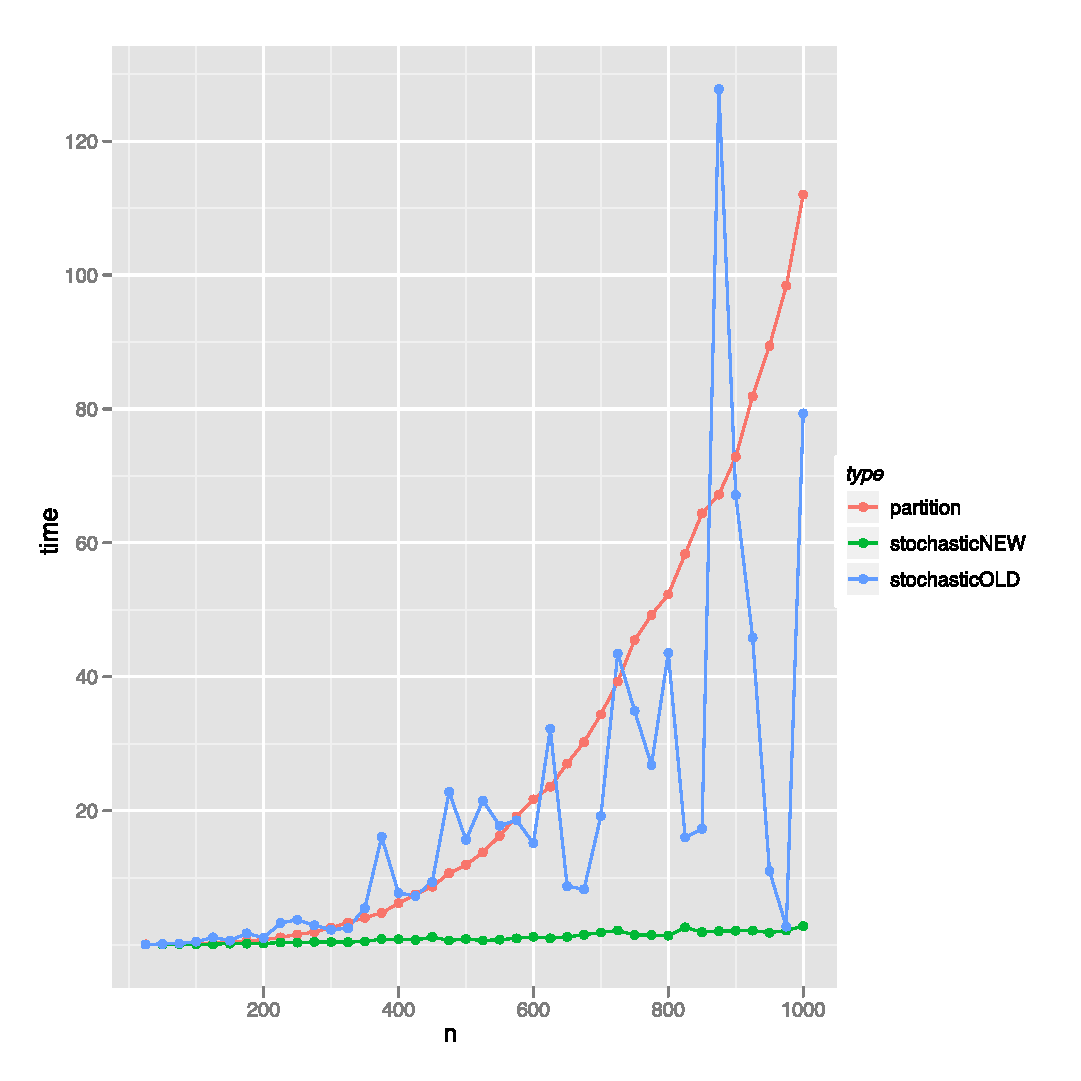
\includegraphics[width=\textwidth]{stochOldvNew.eps}
\caption{A comparison of the computation time between the partition
  function computation, and stochastic tracebacks of 1000 samples with
  the Old algorithm and the new algorithm. The new algorithm is much
  faster.}
\label{fig:stochOvN}
\end{figure}
\begin{figure}[t]
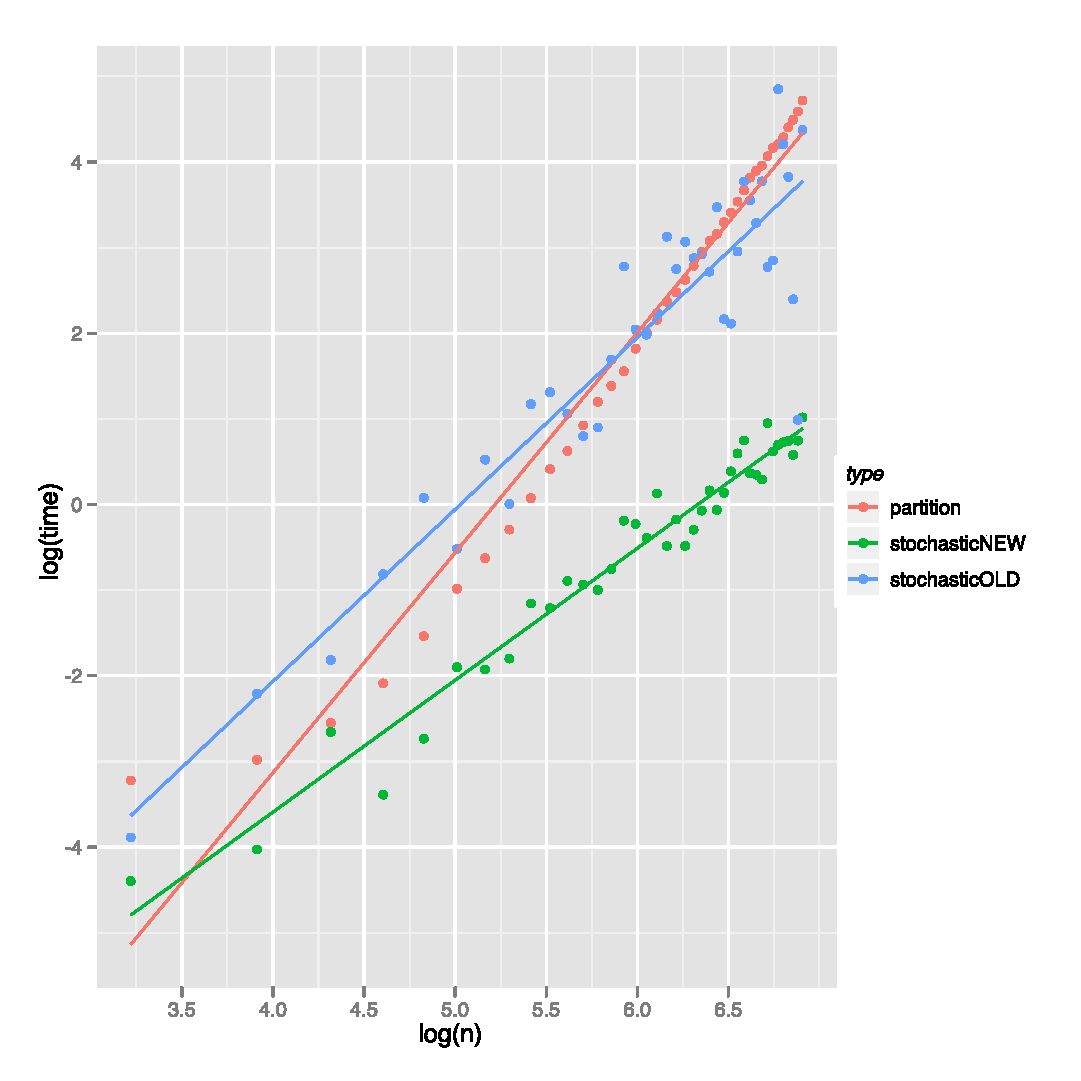
\includegraphics[width=\textwidth]{stochloglog.eps}
\caption{Log-Log plots of the timings in Figure
  \ref{fig:stochOvN}. The new stochastic algorithm slope is slightly
  higher than 1, but not much. }
\label{fig:stochLogLog}
\end{figure}
A good question to ask would be, how do we know that this new
algorithm is outputting structures with the correct
probabilities. Verification plot Figure \ref{fig:stochV} attempts to answer that
question.
\begin{figure}
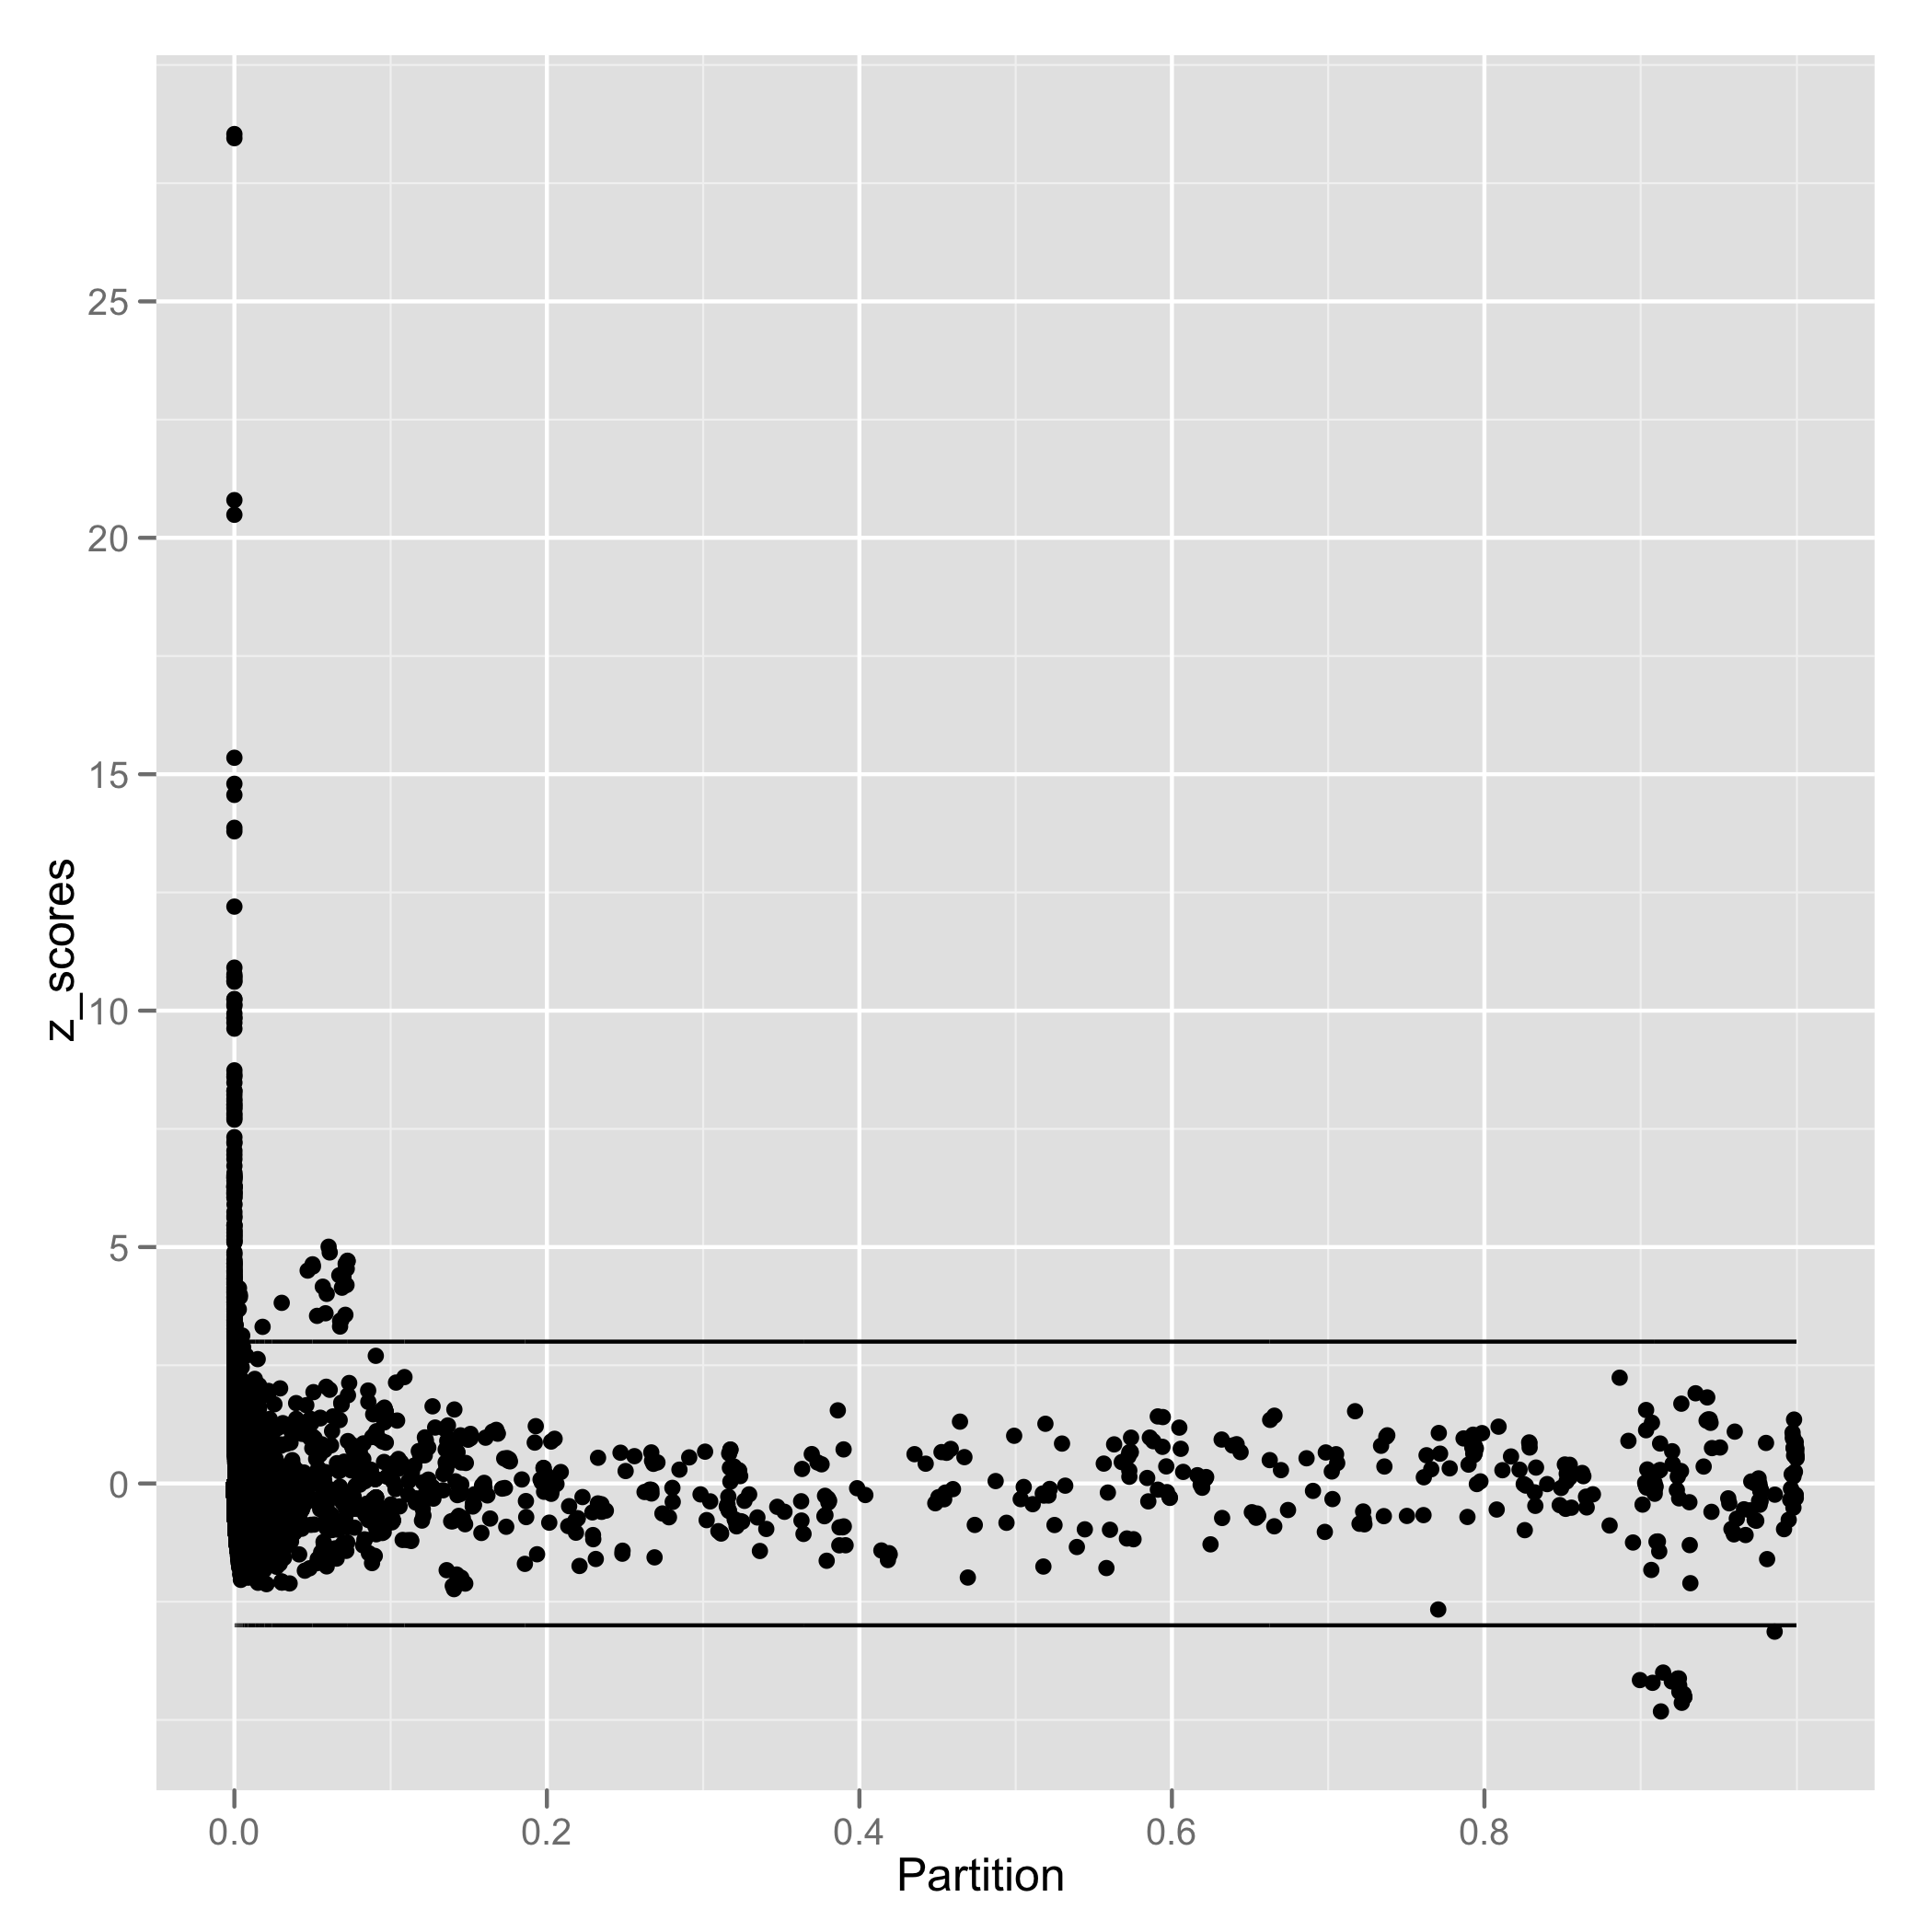
\includegraphics[width=\textwidth]{newzscores.png}
\caption{A plot of the difference between the partition function
  probability and the stochastic traceback probability of a base pair
  according to the new algorithm. According to the number of states,
  there should be 30 states above 0 probability that cross the
  horizontal lines, there are less than 30.}
\label{fig:stochV}
\end{figure}

What we would expect to see from these plots, is that for a given
base, we would expect to see it pair with other bases with
probabilities given by the partition function as one can see. Of
course there is sampling error, so each bin represents a sampling from
a Bernoulli distribution. For $n^2$ samples, we would expect [Todo: find
out what error we expect] error. The number of samples that violate
the bounds, do not deviate much from what we would expect from doing
$n^2$ experiments, so I think we can confidently say that the new
algorithm is making the correct computation.

%[TODO: Add demonstration of full RAM sampling]

\section{Conclusion}

The stochastic traceback algorithm can be sped up to allow large
amounts of sampling such that the limiting computation factor is
memory, not time. The applications of this improvement are that
statistical algorithms like Ding \& Lawrence \cite{ding2004sfold}
\cite{ding2005rna} can minimize their statistical error. Nestor
\cite{aalbertsNestor} benefits greatly from these improvements because
more structures mean more branches to the tree. In general the
algorithm is useful because it removes unnecessary computation that
was done before.
